\section{Results}

The circuit obtained in the previous section can be applied to a system of 4 qubits several times to perform a random walk. 
Fig. 3 shows the results of a 100 steps random walks, obtained by applying the circuit defined in Fig.2 100 times. 

\begin{figure}[h!]
    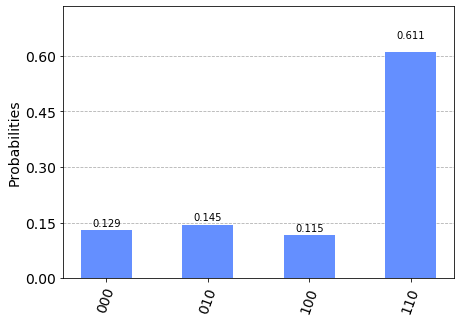
\includegraphics[scale=0.4]{img/100_steps_walk.png}
    \caption{results of a 100 step coined quantum walk}
    \centering
\end{figure}

As we can notice in Fig.4 the probabilities of finding the walker in a given position are 
quite asymmetrical and also, since we started from an even number, odd numbers have zero probability of 
being measured. Differently from classical, we can 
see a true randomness behavior different from a Gaussian distribution that we will observe in a 
classical random walk. The image below taken from \cite{Kendon2004} shows a comparison between
the gaussian distribution of classical systems and the distribution observed for the quantum after 
100 step of the walk.

\begin{figure}[h!]
    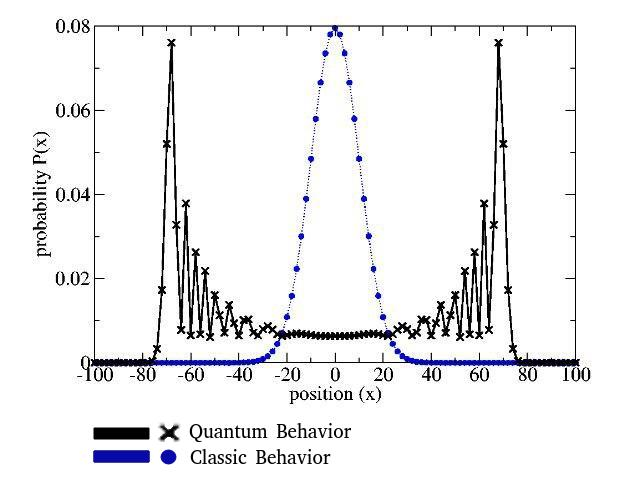
\includegraphics[scale=0.5]{img/dist.jpg}
    \caption{comparison of distribution of a 100 step random walk between classical and quantum}
    \centering
\end{figure}

This means that the walker can pass through or be in an odd(even) position but the probability to measure the Walker in a odd(even) position starting 
from an even(odd) position after 100 steps of the walk is very close to zero.  
An explanation of this behavior can be found in \cite{Kempe_2003}, this strange behavior is due to the Hadamard coin, which treats the two direction (left, right) differently. 
Considering the two states $\ket{\uparrow }$ and $\ket{\downarrow }$ this coin multiply the phase 
by -1 only in case of $\ket{\downarrow }$ inducing more cancellations of the right-wards paths.

The asymmetrical behavior can be modified by changing the initial state or 
changing the coin or balance the Hadamard coin, a more formal description of this behavior is showed in \cite{6812670}.

This particular distribution is interesting since shows that quantum can achieve a true randomness, while classical computer simulate with algorithms this random behavior. 